\chapter{Data Acquisition System}
\label{ch:fddp-daq}

%%%%%%%%%%%%%%%%%%%%%%%%%%%%%%%%%%%%%%%%%%%%%%%%%%%%%%%%%%%%%%%%%%%%
\section{Data Acquisition System (DAQ) Overview}
\label{sec:fddp-daq-ov}


%%%%%%%%%%%%%%%%%%%%%%%%%%%%%%%%%
\subsection{Introduction}
\label{sec:fddp-daq-intro}

The Data Acquisition System provides ...
The system includes (whatever it includes), as shown in Figure.... 

\fixme{Include an image of the overall system, indicating its parts. Show how the system fits into the overall detector.}

The operating principle is illustrated in Figure~\ref{figure-label}... (add figure)

\begin{dunefigure}[DP DAQ Overview]{fig:dp-daq-overview}
  {A generalized overview of high-level far detector \dword{daq}
    components showcasing the \dword{dp} \dword{detmodule}. 
    The electronics digitizes the detector signals and sends the data
    to the DAQ \dword{fe} readout hardware which sends the data to the
    \dword{fe} computing data receiver.
    The receiver sends the data to the \dword{ringbuffer} which is of
    sufficient size to retain the data long enough for a
    \dword{trigcommand} formed from the data itself to return.
    The receiver is also responsible to send out \dwords{trigcandidate} to the
    \dword{mtl} as input to forming a \dword{trigcommand}. 
    The \dword{mtl} forwards notification of this trigger process
    and accepts external \dwords{trigcandidate} from the \dword{gtl}.
    \Dwords{trigcommand} are then sent to the \dlong{eb} which queries
    the appropriate \dword{fe} computing units, aggregates the
    returned data and writes it to the \dword{diskbuffer} which is the
    interface to the Offline.}
  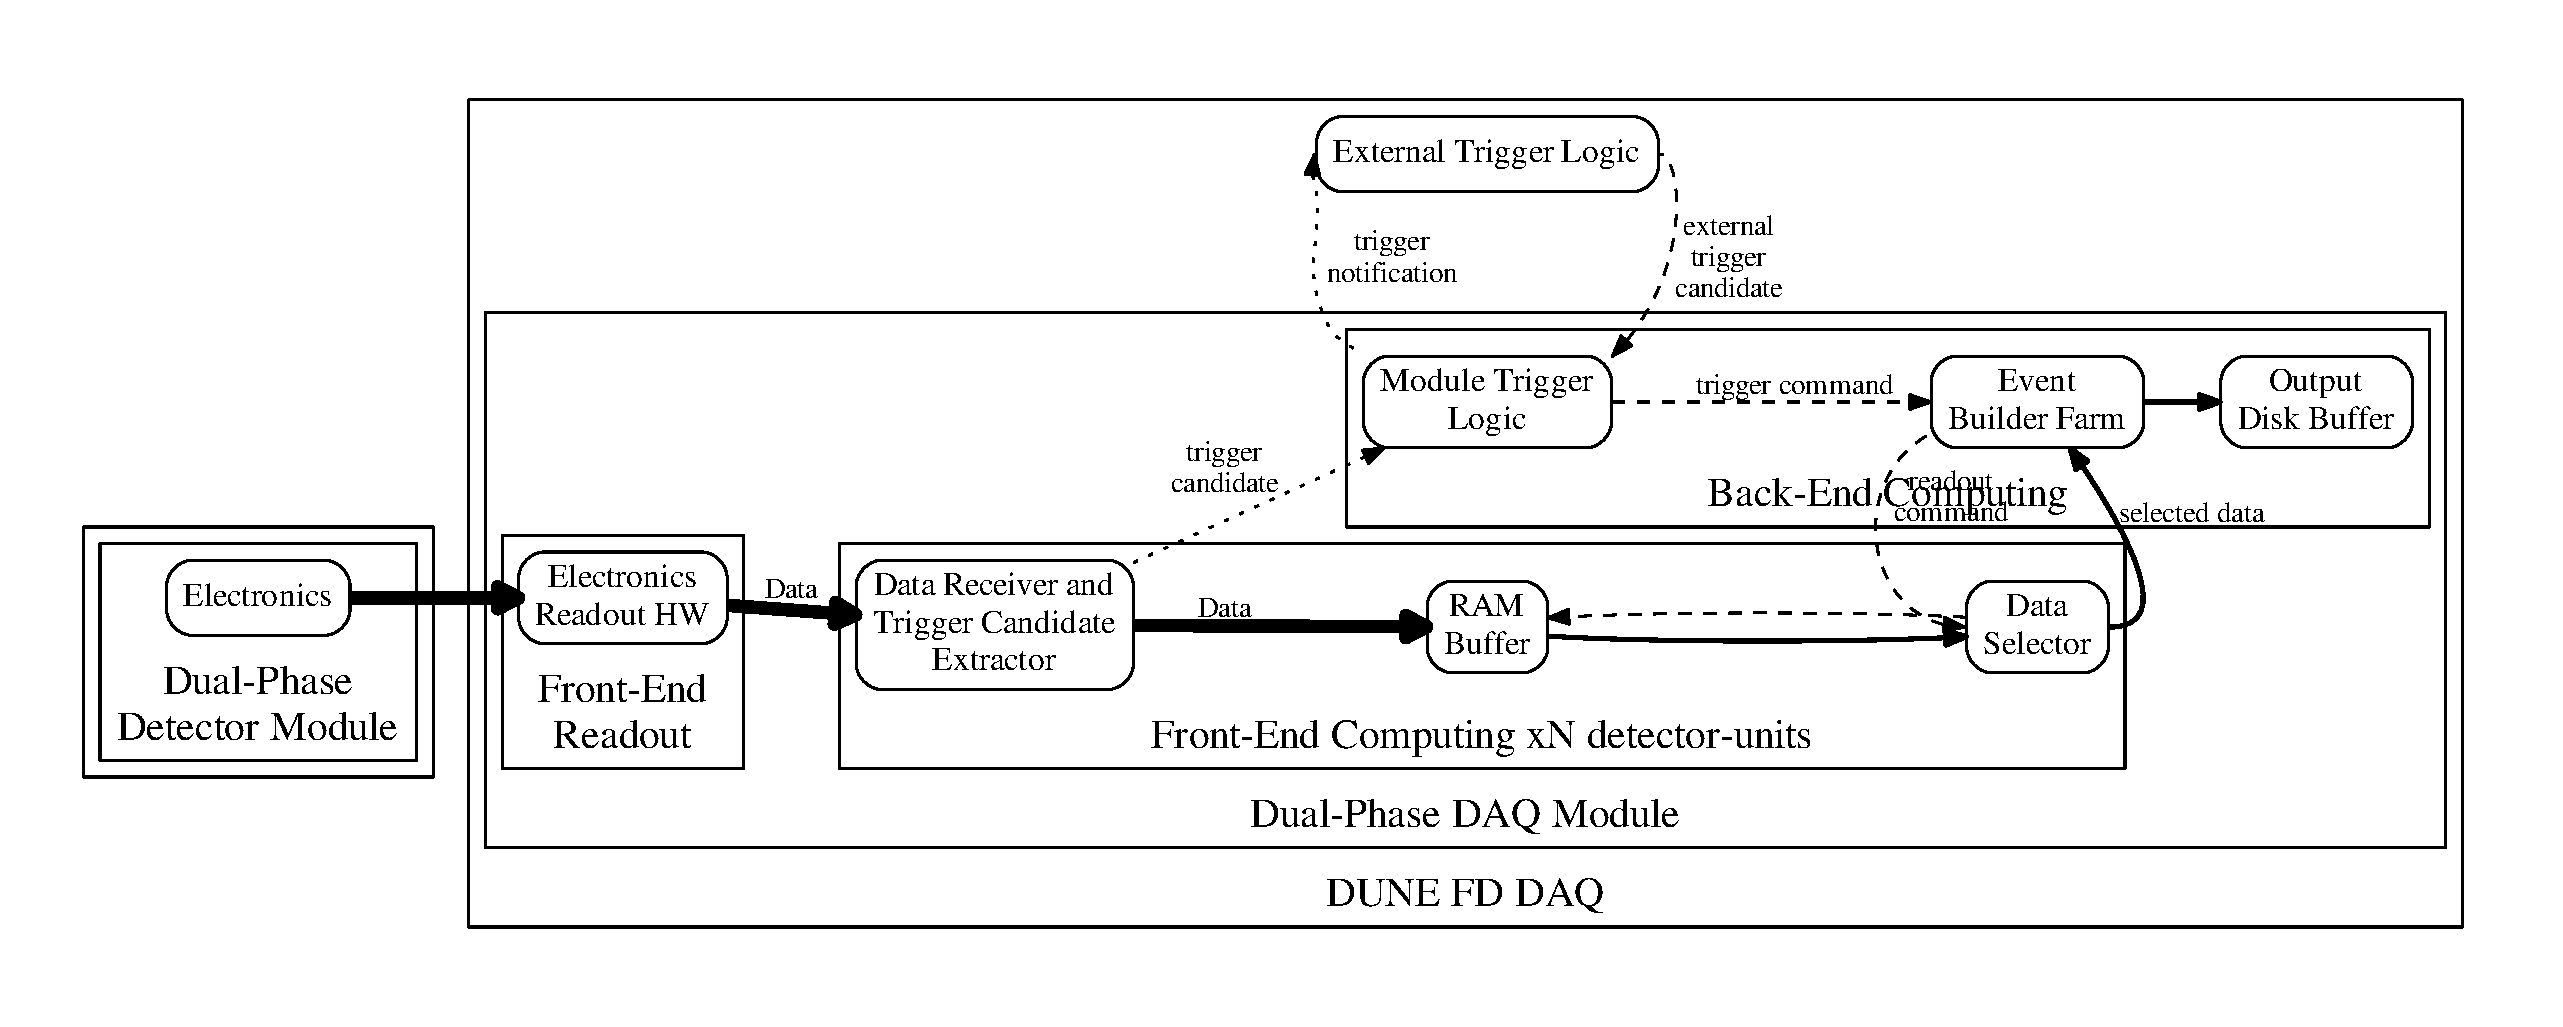
\includegraphics[width=0.8\textwidth]{daq-overview-dp.pdf}%
\end{dunefigure}


%%%%%%%%%%%%%%%%%%%%%%%%%%%%%%%%%%%%%
\subsection{Design Considerations}
\label{sec:fddp-daq-des-consid}


The Data Acquisition System design must enable... 
...

\fixme{Anne suggests: Within this section add ref to requirements document  when it's ready, and maybe list the most important half dozen in a table here). E.g.,}  

See Table~\ref{tab:dp-daqphysicsparams} for a list of the physics parameters that drive the design...

\begin{dunetable}
[Important parameters for the DAQ system design]
{p{0.8\textwidth}}
{tab:dp-daqphysicsparams}
{Important parameters for the DAQ system design}   
Parameter  \\ \toprowrule
  \\ \colhline
   \\ \colhline
 ...\\ 
\end{dunetable}
\fixme{By the end of the volume, for every requirement listed in this section, there should exist an explanation of how it will be satisfied.}


%%%%%%%%%%%%%%%%%%%%%%%%%%%%%%%%
\subsection{Scope}
\label{sec:fddp-daq-scope}

The scope of the Data Acquisition System includes the continued procurement of materials for, and the fabrication, testing, delivery and installation of the following systems: 

\fixme{Whatever the items are...}

\begin{itemize}
\item Photomulitplier tubes 
\item  ...
\end{itemize}



%%%%%%%%%%%%%%%%%%%%%%%%%%%%%%%%%%%%%%%%%%%%%%%%%%%%%%%%%%%%%%%%%%%%
\section{DAQ Design}
\label{sec:fddp-daq-design}


\fixme{Include an image of the subsystem, indicating its parts. Show how the system fits into the overall system).}

\fixme{not sure what subsections are needed: ?}

%%%%%%%%%%%%%%%%%%%%%%%%%%%%%%%%%%%
\subsection{??}
\label{sec:fddp-daq-??}

%%%%%%%%%%%%%%%%%%%%%%%%%%%%%%%%%%%
\subsection{Quality Assurance}
\label{sec:fddp-daq-qa}




%%%%%%%%%%%%%%%%%%%%%%%%%%%%%%%%%%%%%%%%%%%%%%%%%%%%%%%%%%%%%%%%%%%%
\section{Production and Assembly}
\label{sec:fddp-daq-prod-assy}

%%%%%%%%%%%%%%%%%%%%%%%%%%%%%%%%%%
\subsection{}
\label{sec:fddp-daq-?}

%%%%%%%%%%%%%%%%%%%%%%%%%%%%%%%%%%
\subsection{?}
\label{sec:fddp-daq-??}


%%%%%%%%%%%%%%%%%%%%%%%%%%%%%%%%%%
\subsection{Tooling}
\label{sec:fddp-daq-tooling}


%%%%%%%%%%%%%%%%%%%%%%%%%%%%%%%%%
\subsection{Assembly Procedures}
\label{sec:fddp-daq-assy}



%%%%%%%%%%%%%%%%%%%%%%%%%%%%%%%%%%%%%%%%%%%%%%%%%%%%%%%%%%%%%%%%%%%%
\section{Interfaces}
\label{sec:fddp-daq-intfc}

\fixme{Include an image of each interface in appropriate section.}

\fixme{Add in appropriate subsections for the pieces that the Data Acquisition System interfaces with. These initial ones may not be right.}

%%%%%%%%%%%%%%%%%%%%%%%%%%%%%%%%%%%
\subsection{TPC Electronics}
\label{sec:fddp-daq-intfc-elec}


%%%%%%%%%%%%%%%%%%%%%%%%%%%%%%%%%%%
\subsection{}
\label{sec:fddp-daq-intfc-?}


%%%%%%%%%%%%%%%%%%%%%%%%%%%%%%%%%%%%%%%%%%%%%%%%%%%%%%%%%%%%%%%%%%%%
\section{Installation, Integration and Commissioning}
\label{sec:fddp-daq-install}

%%%%%%%%%%%%%%%%%%%%%%%%%%%%%%%%%%%%
\subsection{Transport and Handling}
\label{sec:fddp-daq-install-transport}


%%%%%%%%%%%%%%%%%%%%%%%%%%%%%%%%%%%
\subsection{Integration with (electronics, ???)}
\label{sec:fddp-daq-install-pd-???}


%%%%%%%%%%%%%%%%%%%%%%%%%%%%%%%%%%%
\subsection{Calibration?}
\label{sec:fddp-daq-install-calib}



%%%%%%%%%%%%%%%%%%%%%%%%%%%%%%%%%%%%%%%%%%%%%%%%%%%%%%%%%%%%%%%%%%%%
\section{Quality Control}
\label{sec:fddp-daq-qc}

%%%%%%%%%%%%%%%%%%%%%%%%%%%%%%%%%%%%
\subsection{Protection and Assembly (Local)}
\label{sec:fddp-daq-qc-local}


%%%%%%%%%%%%%%%%%%%%%%%%%%%%%%%%%%%
\subsection{Post-factory Installation (Remote)}
\label{sec:fddp-daq-qc-remote}





%%%%%%%%%%%%%%%%%%%%%%%%%%%%%%%%%%%%%%%%%%%%%%%%%%%%%%%%%%%%%%%%%%%%
\section{Safety}
\label{sec:fddp-daq-safety}

%%%%%%%%%%%%%%%%%%%%%%%%%%%%%%%%%%%
% add subsections and labels if needed \subsection{}
%\label{sec:fddp-daq-safety-}


%%%%%%%%%%%%%%%%%%%%%%%%%%%%%%%%%%
%\subsection{}
%\label{sec:fddp-daq-safety}



%%%%%%%%%%%%%%%%%%%%%%%%%%%%%%%%%%%%%%%%%%%%%%%%%%%%%%%%%%%%%%%%%%%%
\section{Organization and Management}
\label{sec:fddp-daq-org}

%%%%%%%%%%%%%%%%%%%%%%%%%%%%%%%%%%%
\subsection{DAQ Consortium Organization}
\label{sec:fddp-daq-org-consortium}


%%%%%%%%%%%%%%%%%%%%%%%%%%%%%%%%%%
\subsection{Planning Assumptions}
\label{sec:fddp-daq-org-assmp}


%%%%%%%%%%%%%%%%%%%%%%%%%%%%%%%%%%%
\subsection{WBS and Responsibilities}
\label{sec:fddp-daq-org-wbs}

%%%%%%%%%%%%%%%%%%%%%%%%%%%%%%%%%%
\subsection{High-level Cost and Schedule}
\label{sec:fddp-daq-org-cs}














